\documentclass{standalone}
\usepackage{tikz}
\usetikzlibrary{patterns, positioning}
\usepackage[sfdefault]{ClearSans} %% option 'sfdefault' activates Clear Sans as the default text font
\usepackage[T1]{fontenc}

\begin{document}
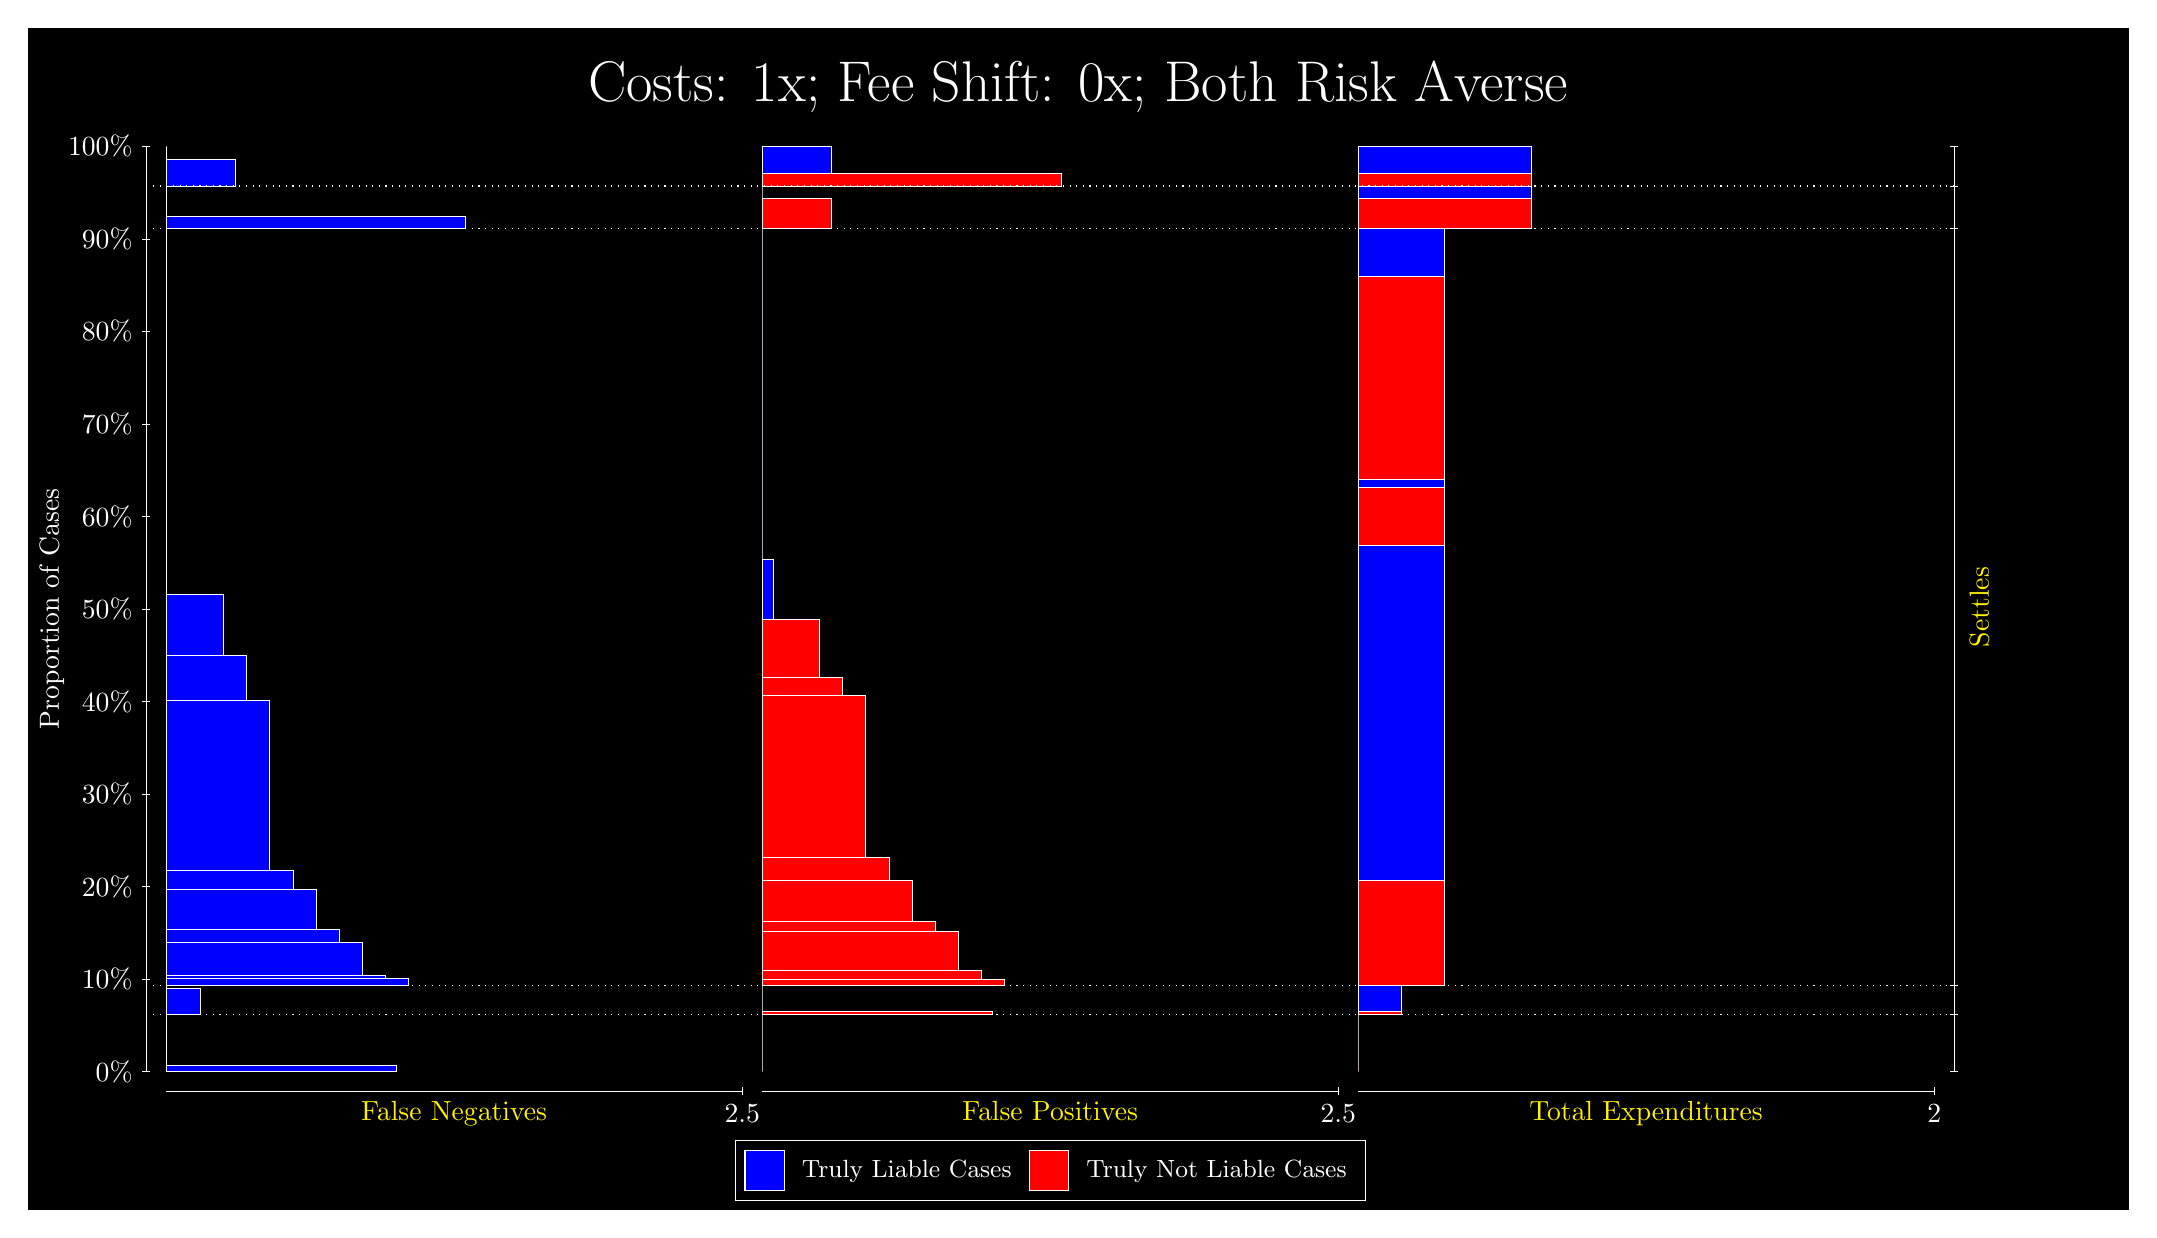
\begin{tikzpicture}
\draw[fill=black] (0,0) rectangle (26.667,15);
\draw[text=white] (0,13.5) rectangle (26.667,15) node[midway] {\huge Costs: 1x; Fee Shift: 0x; Both Risk Averse};
\draw[white, very thin] (1.5,1.75) -- (1.5,13.5);
\node[rotate=90, text=white, anchor=center] at (0.3, 7.625) {Proportion of Cases};
\draw[white, very thin] (1.45,1.75) -- (1.55,1.75);
\node[text=white, anchor=east] at (1.45, 1.75) {0\%};
\draw[white, very thin] (1.45,2.925) -- (1.55,2.925);
\node[text=white, anchor=east] at (1.45, 2.925) {10\%};
\draw[white, very thin] (1.45,4.1) -- (1.55,4.1);
\node[text=white, anchor=east] at (1.45, 4.1) {20\%};
\draw[white, very thin] (1.45,5.275) -- (1.55,5.275);
\node[text=white, anchor=east] at (1.45, 5.275) {30\%};
\draw[white, very thin] (1.45,6.45) -- (1.55,6.45);
\node[text=white, anchor=east] at (1.45, 6.45) {40\%};
\draw[white, very thin] (1.45,7.625) -- (1.55,7.625);
\node[text=white, anchor=east] at (1.45, 7.625) {50\%};
\draw[white, very thin] (1.45,8.8) -- (1.55,8.8);
\node[text=white, anchor=east] at (1.45, 8.8) {60\%};
\draw[white, very thin] (1.45,9.975) -- (1.55,9.975);
\node[text=white, anchor=east] at (1.45, 9.975) {70\%};
\draw[white, very thin] (1.45,11.15) -- (1.55,11.15);
\node[text=white, anchor=east] at (1.45, 11.15) {80\%};
\draw[white, very thin] (1.45,12.325) -- (1.55,12.325);
\node[text=white, anchor=east] at (1.45, 12.325) {90\%};
\draw[white, very thin] (1.45,13.5) -- (1.55,13.5);
\node[text=white, anchor=east] at (1.45, 13.5) {100\%};

\draw[white, very thin] (24.457,1.75) -- (24.457,13.5);
\draw[white, very thin] (24.407,1.75) -- (24.507,1.75);
\node[anchor=west] at (24.407, 1.75) {};
\draw[white, very thin] (24.407,2.4788) -- (24.507,2.4788);
\node[anchor=west] at (24.407, 2.4788) {};
\draw[white, very thin] (24.407,2.8431) -- (24.507,2.8431);
\node[anchor=west] at (24.407, 2.8431) {};
\draw[white, very thin] (24.407,12.457) -- (24.507,12.457);
\node[anchor=west] at (24.407, 12.457) {};
\draw[white, very thin] (24.407,12.996) -- (24.507,12.996);
\node[anchor=west] at (24.407, 12.996) {};
\draw[white, very thin] (24.407,13.5) -- (24.507,13.5);
\node[anchor=west] at (24.407, 13.5) {};

\draw[white, very thin, fill=blue] (1.75,1.75) rectangle (4.6775,1.8267);
\draw[white, very thin, fill=red] (1.75,1.8267) rectangle (1.75,2.4788);
\draw[white, very thin, fill=blue] (1.75,2.4788) rectangle (2.1891,2.8048);
\draw[white, very thin, fill=red] (1.75,2.8048) rectangle (1.75,2.8431);
\draw[white, very thin, fill=blue] (1.75,2.8431) rectangle (4.8239,2.9395);
\draw[white, very thin, fill=blue] (1.75,2.9395) rectangle (4.5312,2.9762);
\draw[white, very thin, fill=blue] (1.75,2.9762) rectangle (4.2384,3.3882);
\draw[white, very thin, fill=blue] (1.75,3.3882) rectangle (3.9457,3.5504);
\draw[white, very thin, fill=blue] (1.75,3.5504) rectangle (3.6529,4.0688);
\draw[white, very thin, fill=blue] (1.75,4.0688) rectangle (3.3602,4.3017);
\draw[white, very thin, fill=blue] (1.75,4.3017) rectangle (3.0674,6.4685);
\draw[white, very thin, fill=blue] (1.75,6.4685) rectangle (2.7746,7.0402);
\draw[white, very thin, fill=blue] (1.75,7.0402) rectangle (2.4819,7.8109);
\draw[white, very thin, fill=red] (1.75,7.8109) rectangle (1.75,12.457);
\draw[white, very thin, fill=blue] (1.75,12.457) rectangle (5.5558,12.617);
\draw[white, very thin, fill=red] (1.75,12.617) rectangle (1.75,12.996);
\draw[white, very thin, fill=blue] (1.75,12.996) rectangle (2.6283,13.34);
\draw[white, very thin, fill=red] (1.75,13.34) rectangle (1.75,13.5);
\draw[white, very thin, fill=red] (9.3189,1.75) rectangle (9.3189,2.4021);
\draw[white, very thin, fill=blue] (9.3189,2.4021) rectangle (9.3189,2.4788);
\draw[white, very thin, fill=red] (9.3189,2.4788) rectangle (12.246,2.5171);
\draw[white, very thin, fill=blue] (9.3189,2.5171) rectangle (9.3189,2.8431);
\draw[white, very thin, fill=red] (9.3189,2.8431) rectangle (12.393,2.9259);
\draw[white, very thin, fill=red] (9.3189,2.9259) rectangle (12.1,3.0371);
\draw[white, very thin, fill=red] (9.3189,3.0371) rectangle (11.807,3.5304);
\draw[white, very thin, fill=red] (9.3189,3.5304) rectangle (11.515,3.6643);
\draw[white, very thin, fill=red] (9.3189,3.6643) rectangle (11.222,4.1774);
\draw[white, very thin, fill=red] (9.3189,4.1774) rectangle (10.929,4.4727);
\draw[white, very thin, fill=red] (9.3189,4.4727) rectangle (10.636,6.5241);
\draw[white, very thin, fill=red] (9.3189,6.5241) rectangle (10.344,6.7559);
\draw[white, very thin, fill=red] (9.3189,6.7559) rectangle (10.051,7.4891);
\draw[white, very thin, fill=blue] (9.3189,7.4891) rectangle (9.4652,8.2598);
\draw[white, very thin, fill=blue] (9.3189,8.2598) rectangle (9.3189,12.457);
\draw[white, very thin, fill=red] (9.3189,12.457) rectangle (10.197,12.836);
\draw[white, very thin, fill=blue] (9.3189,12.836) rectangle (9.3189,12.996);
\draw[white, very thin, fill=red] (9.3189,12.996) rectangle (13.125,13.155);
\draw[white, very thin, fill=blue] (9.3189,13.155) rectangle (10.197,13.5);
\draw[white, very thin, fill=red] (16.888,1.75) rectangle (16.888,2.4021);
\draw[white, very thin, fill=blue] (16.888,2.4021) rectangle (16.888,2.4788);
\draw[white, very thin, fill=red] (16.888,2.4788) rectangle (17.437,2.5171);
\draw[white, very thin, fill=blue] (16.888,2.5171) rectangle (17.437,2.8431);
\draw[white, very thin, fill=red] (16.888,2.8431) rectangle (17.986,4.1774);
\draw[white, very thin, fill=blue] (16.888,4.1774) rectangle (17.986,8.4379);
\draw[white, very thin, fill=red] (16.888,8.4379) rectangle (17.986,9.171);
\draw[white, very thin, fill=blue] (16.888,9.171) rectangle (17.986,9.2674);
\draw[white, very thin, fill=red] (16.888,9.2674) rectangle (17.986,11.846);
\draw[white, very thin, fill=blue] (16.888,11.846) rectangle (17.986,12.457);
\draw[white, very thin, fill=red] (16.888,12.457) rectangle (19.083,12.836);
\draw[white, very thin, fill=blue] (16.888,12.836) rectangle (19.083,12.996);
\draw[white, very thin, fill=red] (16.888,12.996) rectangle (19.083,13.155);
\draw[white, very thin, fill=blue] (16.888,13.155) rectangle (19.083,13.5);
\draw[white, dotted] (1.5,2.4788) -- (24.457,2.4788);
\draw[white, dotted] (1.5,2.8431) -- (24.457,2.8431);
\draw[white, dotted] (1.5,12.457) -- (24.457,12.457);
\draw[white, dotted] (1.5,12.996) -- (24.457,12.996);
\draw[white, very thin] (1.75,1.5) -- (9.0689,1.5);
\node[text=yellow, anchor=north] at (5.4094, 1.5) {False Negatives};
\draw[white, very thin] (9.0689,1.45) -- (9.0689,1.55);
\node[text=white, anchor=north] at (9.0689, 1.45) {2.5};

\draw[white, very thin] (9.3189,1.5) -- (16.638,1.5);
\node[text=yellow, anchor=north] at (12.978, 1.5) {False Positives};
\draw[white, very thin] (16.638,1.45) -- (16.638,1.55);
\node[text=white, anchor=north] at (16.638, 1.45) {2.5};

\draw[white, very thin] (16.888,1.5) -- (24.207,1.5);
\node[text=yellow, anchor=north] at (20.547, 1.5) {Total Expenditures};
\draw[white, very thin] (24.207,1.45) -- (24.207,1.55);
\node[text=white, anchor=north] at (24.207, 1.45) {2};



\node[text=yellow, centered, rotate=90] at (24.777, 7.65) {Settles};



\draw (12.978300999999998,1.5) node[draw=none] (baseCoordinate) {};
\begin{scope}[align=center]
        \matrix[scale=0.5, draw=white, below=0.5cm of baseCoordinate, nodes={draw}, column sep=0.1cm]{
            \node[rectangle, draw, minimum width=0.5cm, minimum height=0.5cm, fill=blue] {}; &
            \node[draw=none, font=\small, text=white] (B) {Truly Liable Cases}; &
            \node[rectangle, draw, minimum width=0.5cm, minimum height=0.5cm, fill=red] {}; &
            \node[draw=none, font=\small, text=white] (B) {Truly Not Liable Cases}; \\
            };
\end{scope}

\end{tikzpicture}
\end{document}